%Auswertung


\section{Wenner-Kartierung}
Die Wenner-Kartierung wurde auf einem 46\,m langen Profil senkrecht zum Basaltgang durchgeführt. In Tabelle \ref{tab:wenner} sind die gemessenen Werte des spezifischen Widerstands mit dem Entsprechenden festgelegten Abstand zu sehen. Die Abstanände
der Messpunkte sind in der Mitte den Profils kleiner gewählt als Außen, da wir dort den Basaltgang vermuten. Aus den Messergebnissen der Magnetik-Messung könnte schon sehr genau abgeschätzt werden wo der Basaltgang liegt.\\
\\
In Abbildung \ref{abb:Wenner} sind die Messergebnisse graphisch dargestellt. Wir gehen davon aus, dass der Basalt eine andere Leitfähigkeit hat als das Umgebungsmaterial und sich also die Magnetischen-Eigenschaften und elektrische Leitfähigkeit 
gleichzeitig ändern. Das ist die Vorraussetzung, dass wir mit Hilfe unserer Ergebnisse aus der Magnetik unser Profil für die Geoelektrik festlegen können und in beiden Versuchen ähnliche Ergebnisse erhalten.\\
Deutlich zu sehen ist ein Maximum des spezifischen Widerstands in der Mitte des Diagramms \ref{abb:Wenner}.
Dies weist darauf hin, dass der Basaltgang wie vermutet in der Mitte unseres Profils liegt. \\
Rechts und Links von dem großen Maximum sind weitere kleinere Nebenmaxima zu erkennen. Da wir den Untergrund nicht genau kennen, können wir nicht mit Sicherheit sagen, um was es sich dabei handelt. Wir vermuten, dass der Basaltgang etwas verwittert 
ist, sich z.B. durch Wasser Risse im Gestein gebildet haben. Hat sich nun zwischen dem Abgespalteten Basalt leitfähiges Material eingelagert, wir an diesen Stellen ein geringerer spezifischer Widerstand gemessen.\\
Da die Nebenmaxima nicht die gleiche höhe haben wie das Maxima in der Mitte ist es auch wahrscheinlich dass der Baslatgang nicht nur durch Risse unterteilt ist. Wir gehen davon aus, dass das Basalt an den Rändern sehr stank verwittert ist und eventuell
nur noch in kleinen Stücken vorliegt.???\\
\\
Grob stimmen unsere Erkenntnisse mit denen der Magnetik überein.




%%%%%%%%%%%%%%%%%%%%%%%%%%%%%%%%%%%%%%%%%
\begin{figure}[h]
\centering
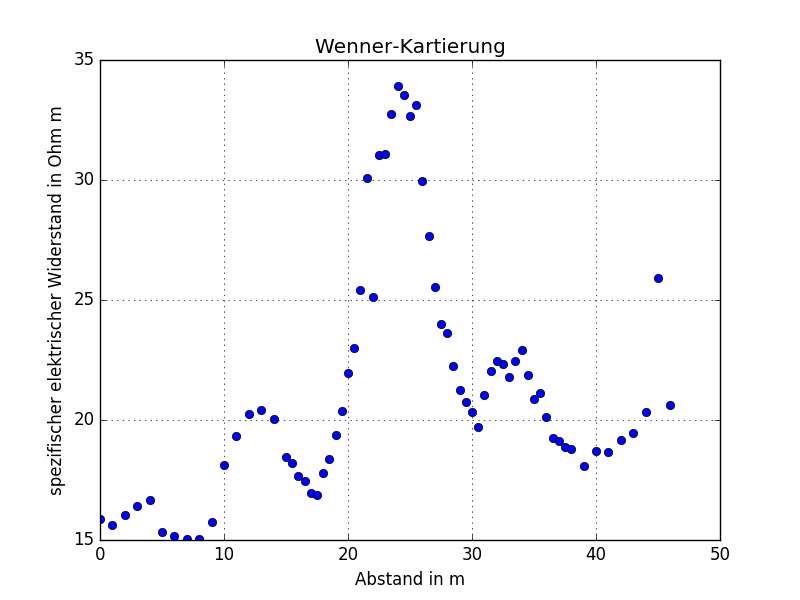
\includegraphics[width=0.6\textwidth]{fig/wennerkartierung.png}
\caption{Diagramm unserer Ergebnisse der Wenner-Kartierung. Der gemessene spezifische Widerstand ist gegen den Abstand zu unserem gewählten Null-Punkt aufgetragen.}
\label{abb:Wenner}
\end{figure}
%%%%%%%%%%%%%%%%%%%%%%%%%%%%%%%%%%%%


%%%%%%%%%%%%%%%%%%%%%%%%%%%%%%%%%%%%%%%%%%%%%%%%%%%%%%%%%%%%%%%%%%%%
\newcolumntype{C}[1]{>{\centering\arraybackslash}m{#1}}
\begin{table}[h]
\centering
\begin{center}
\begin{tabular}[central]{ c | c }
Abstand in m  & Widerstand in Ohm m \\
\hline
0	&	15,873	\\
1	&	15,605	\\
2	&	16,036	\\
3	&	16,431	\\
4	&	16,658	\\
5	&	15,330	\\
6	&	15,155	\\
7	&	15,029	\\
8	&	15,044	\\
9	&	15,765	\\
10	&	18,122	\\
11	&	19,323	\\
12	&	20,270	\\
13	&	20,403	\\
14	&	20,054	\\
15	&	18,457	\\
15.5	&	18,217	\\
16	&	17,687	\\
16.5	&	17,456	\\
17	&	16,948	\\
17.5	&	16,859	\\
18	&	17,779	\\
18.5	&	18,370	\\
19	&	19,392	\\
19.5	&	20,363	\\
20	&	21,945	\\
20.5	&	23,000	\\
21	&	25,416	\\
21.5	&	30,071	\\
22	&	25,125	\\
22.5	&	31,057	\\
23	&	31,101	\\
23.5	&	32,759	\\
24	&	33,908	\\
24.5	&	33,561	\\
25	&	32,673	\\
25.5	&	33,126	\\
26	&	29,951	\\
26.5	&	27,679	\\
27	&	25,546	\\
27.5	&	24,013	\\
28	&	23,626	\\
28.5	&	22,262	\\
29	&	21,232	\\
29.5	&	20,754	\\
30	&	20,354	\\
30.5	&	19,708	\\
31	&	21,024	\\
31.5	&	22,026	\\
32	&	22,442	\\
32.5	&	22,334	\\
33	&	21,789	\\
33.5	&	22,438	\\
34	&	22,927	\\
34.5	&	21,875	\\
35	&	20,880	\\
35.5	&	21,110	\\
36	&	20,109	\\
36.5	&	19,245	\\
37	&	19,105	\\
37.5	&	18,882	\\
38	&	18,774	\\
39	&	18,104	\\
40	&	18,712	\\
41	&	18,659	\\
42	&	19,165	\\
43	&	19,466	\\
44	&	20,332	\\
45	&	25,904	\\
46	&	20,623	\\
\end{tabular}
\caption{Abstände von alles gefundenen Stufen in den Plots aus Abb. \ref{abb:GoldPlt}}
\label{tab:wenner}
\end{center}
\end{table}
%%%%%%%%%%%%%%%%%%%%%%%%%%%%%%%%%%%%%%%%%%%%%%%%%%%%%%%%%%%%%%%%%%%%


\section{Tomographie}

In Abbildung \ref{abb:Tomographie} sind die Ergebnisse der Tomographie-Messung zu sehen. Die obere Abbildung zeigt die von uns gemessenen Werte für den scheinbaren spezifischen Widerstand. Die Inversion der Werte, also ein Modell wie der Untergrund 
wirklich aussehen könnte ist im unteren Diagramm zu sehen. In der Mitte ist dargestellt, welche Widerstandswerte man gemessen hätte, wenn der Untergrund dem berecneten Modell entsprechen würde.\\
Die beiden oberen Diagramme sind sehr ähnlich, fast identisch. Das bedeutet dass, das berechnete Modell unsere gemessenen Werte sehr gut beschreibt. \\
\\
Bei dem Abstand 13 m ist eine sehr starke Anomalie von ca.$ \SI{ 300}{\Omega m}$. Die Anomalie ist jedoch sehr klein und oberflächennah. Links davon ist eine zweite sehr deutliche Anomalie zu sehen, die, in dem gemessenen Bereich,
mit zunehmender Tiefe größer wird. Der spezifische Widerstand ist hier aber nur maximal etwa $\SI{100}{\Omega m}$. \\
Etwa $\SI{2}{m}$ entfernt von der stärksten Anomalie, bei  $\SI{14}{m}$ beginnt eine dritte, oberflächennahe Anomalie. \\
Beim Vergleich mit den Ergebnissen der Wennerkartierung finden wir größe Ähnlichkeiten. Die Tomographie deutet ebenso wie die Wennerkartierung darauf hin, das der Basaltgang an der gemessenen Stelle grob in drei Teile unterteilt werden kann. 
Diese können wir jetzt aber besser lokalisieren.\\
Dort, wo im Tomographie-Modell der größte spezifische Widerstand zu sehen ist, ist auch das globale Maximum der bei der Wenner-Kartierung. Die beiden Nebenmaxima in Abbildung \ref{abb:Wenner}
sind etwa an der gleichen Stelle wie die zwei kleineren Anomalien der Tomographie. \\ 
Allerdings sollte hier noch beachtet werden, dass die Wennerkartierung in einer Tiefe von $\SI{5}{m}$ vorgenommen wurde. Die Tomographie an ihrem tiefsten Punkt aber nur $\SI{5}{m}$ in die Tiefe geht.
In der Tomographie sehen wir aber dass, die Differenz der stärksten Anomalie und den Nebenmaxima fast $\SI{200}{\Omega m}$ beträgt, was bei einer Skala von $\SI{0}{\Omega m}- \SI{300}{\Omega m}$ sehr viel ist. 
Daher gehen wir davon aus, dass diese Anomalie die Messung der Wennerkartierung stark beeinflusst und dem Maximum in Abbildung \ref{abb:Wenner} entspricht.\\
Diese Annahme wurde überprüft, indem man die Ortsangaben der beiden Diagramme verglichen haben. Leider passt die Wennerkartierung hier nicht mehr gut zur Tomographie. Vermutlich haben die Anomalien in den oberen Schichten wirklich kaum Einfluss auf die Wennerkartierung. Da wir diese in 5\,m Tiefe durchgeführt haben, und das Tomographie-Model eben hier aufhört können wir die beiden Methoden eigentlich nicht vergleichen.


Wir gehen davon aus, dass alle Erhöhungen des spezifische Widerstands verursacht werden. 


%%%%%%%%%%%%%%%%%%%%%%%%%%%%%%%%%%%%
\begin{figure}[h]
\centering
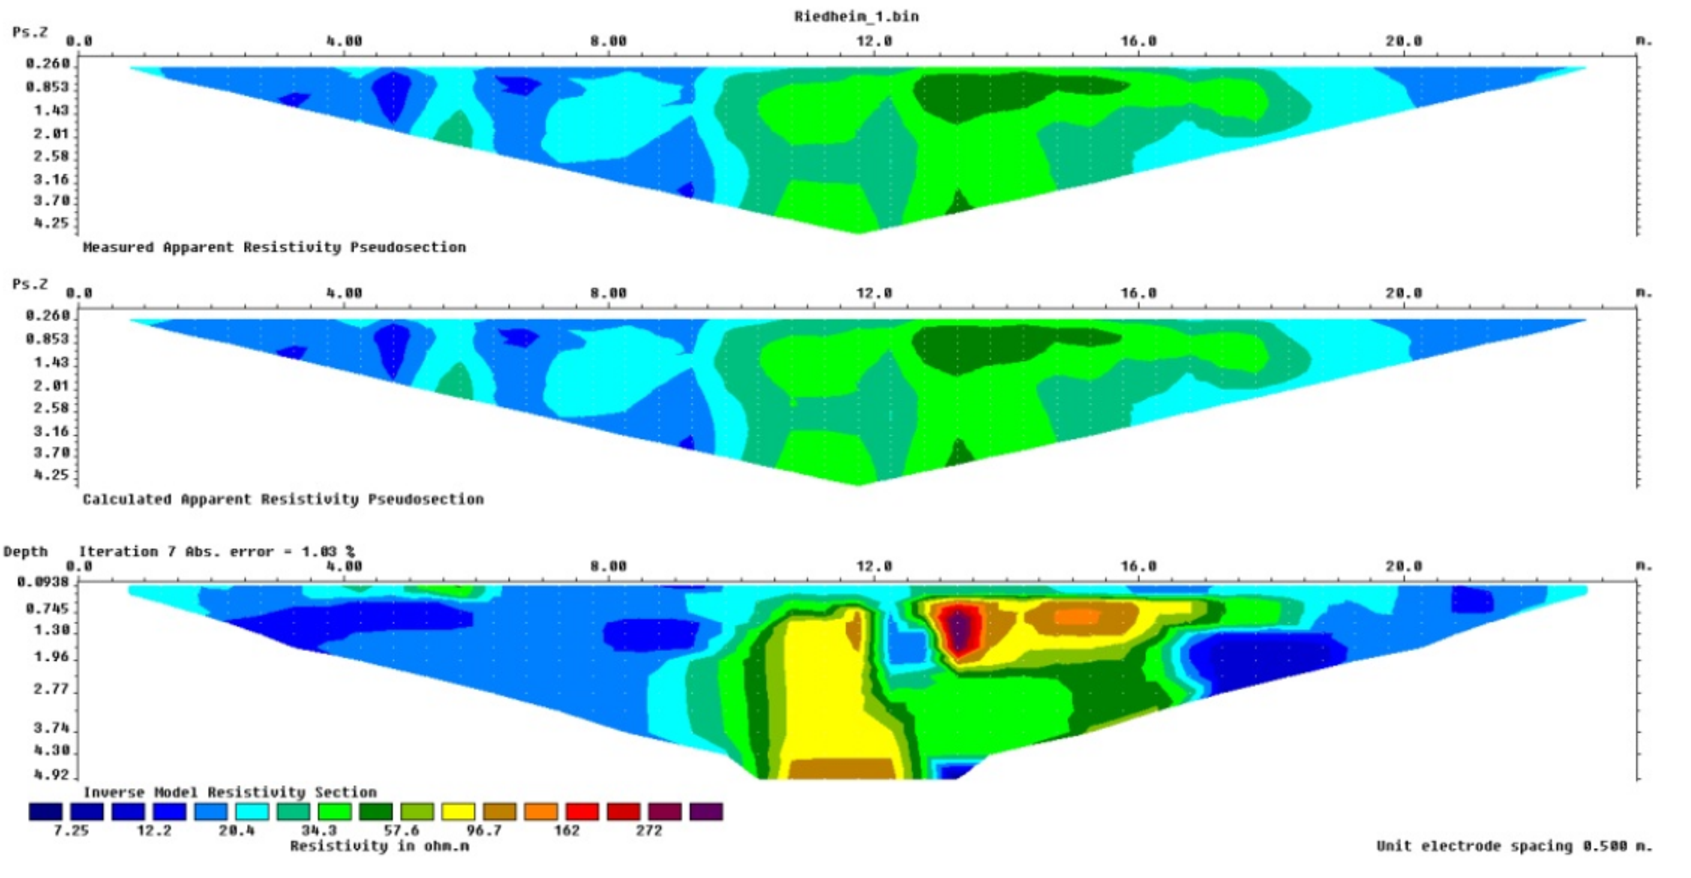
\includegraphics[width=0.85\textwidth]{fig/Tomographie.pdf}
\caption{Tomographie Modell. Als Anfangspunkt der Messung wurde das obere Ende der Profillinie gewählt.}
\label{abb:Tomographie}
\end{figure}
%%%%%%%%%%%%%%%%%%%%%%%%%%%%%%%%%%%%

Die Tomographie ist von 28\,m  bis 51,5\,m positioniert. Die bedeuted, dass der Mittelpunkt der Tomographie, 12\,m, gerade dem Punkt  


\section{Sondierung}
Die Sondierung wurde auf dem Profil ??? durchgeführt. Die Messwerte sind im Anhang zu sehen. Aus ihnen werden mit Hilfe von dem Inversionsprogramm Ipi2win Modelle für die Schichten im Untergrund erstellt. In Abbildung \ref{abb:Schlum1} und \ref{abb:Schlum2} sind die Ergebnisse zu sehen. Die schwarze Kurve ist die Fitkurve durch unsere Messpunkte, in blau ist das Modell des spezifische Widerstands des Untergrunds dargestellt. Die rote Kurve ist der scheinbare spezifische Widerstand, der sich aus diesem Modell ergibt.\\
Als erstes haben wir ein möglichst genauen Model erstellt, mit der Annahme das wir drei Schichten gegeben haben. Das Ergebnis ist in Abbildung \ref{abb:Schlum1} zu sehen. Der Fehler dieses Models lag bei unter 2\%. In Abbildung \ref{abb:SchlumTab1} ist die dazugehörige Tabelle mit dem berechneten spezifischen Widerstand $\rho$, der Dicke $h$ und Tiefe $d$ der jeweiligen Schichten.  Alle drei Werte nehmen mit der Tiefe zu, was sehr plausibel ist. Die erste Schichtgrenze ist in etwa $\SI{5}{cm}$ Tiefe und die zweite schon bei $\SI{43}{cm}$, die dritte erst bei etwa $\SI{8}{m}$. Diese Ergebnisse lassen sich leider nicht mit denen der Seismik vergleichen. 



%%%%%%%%%%%%%%%%%%%%%%%%%%%%%%%%%%%%
\begin{figure}[h]
\centering
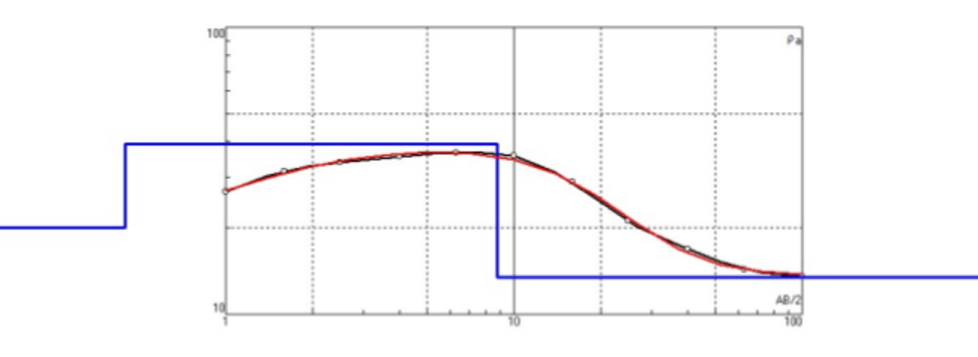
\includegraphics[width=0.8\textwidth]{fig/Schlumberger_3Schichten.pdf}
\caption{Inversionsmodel mit drei Schichten }
\label{abb:Schlum1}
\end{figure}
%%%%%%%%%%%%%%%%%%%%%%%%%%%%%%%%%%%%
%%%%%%%%%%%%%%%%%%%%%%%%%%%%%%%%%%%%
\begin{figure}[h]
\centering
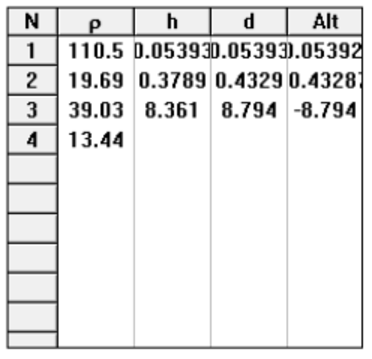
\includegraphics[width=0.3\textwidth]{fig/schlumbergerTabelle.pdf}
\caption{Datem zum Inversionsmodel mit drei Schichten. $roh$ bezeichnet den spezifischen Widerstand in $\Omega$m, $h$ die Schichtdicke in m, $d$ die Schichttiefe in m}
\label{abb:SchlumTab1}
\end{figure}
%%%%%%%%%%%%%%%%%%%%%%%%%%%%%%%%%%%%


Als zweites haben wir die Inversion ohne vorgegebene Maximalzahl der Schichten gemacht. Dabei wurde ein Modell mit 5 Schichten berechnet, welches in Abbildung \ref{abb:Schlum2} zu sehen ist. Die Tabelle mit den Entsprechenden Werten ist in Abbildung \ref{abb:SchlumTab2} gegeben. \\
Die erste Schichtgrenze liegt bei $\SI{60}{cm}$. Beim bohren mit Franz stießen wir in dieser Tiefe ebenfalls auf eine Schichtgrenze, zu der reinen Erde an der Oberfläche kamen viele Kieselsteine. Wenn wir davon ausgehen, dass sich damit auch die Leitfähigkeit des Untergrunds ändert, ist diese Schichtgrenze die selbe und wir haben sie durch Bohrung nachgewiesen.\\
  
In $\SI{2,62}{m}$ Tiefe haben wir eine Weitere Schichtgrenze. Interessanterweise haben wir in der Seismik in einer Tiefe von etwa $\SI{3,4 }{m}$ ebenfalls eine Schichtgrenze gefunden. Die mit der Geoelektrik bestimmte Schichtgrenze liegt also noch im Fehlerbereich dieser Schichtgrenze. 
Gehen wir davon aus, das sich hier die Seismischen und Geoelektrischen Eigenschaften des Untergrunds gleichzeitig ändern, haben wir mit dieser Messung das Ergebnis der Seismikmessung bestätigt. 
Weitere Schichtgrenzen befinden sich in $\SI{1,3}{m}$, $\SI{5,5}{m}$ und $\SI{24}{m}$ Tiefe. Bei der 4. Schichtgrenze nimmt der spezifische Widerstand stark zu und bei der 5. Schichtgrenze sinkt sie auf einen niedrigeren Wert als den der ersten Schichten. Dies dann damit erklärt werden dass hier der Grundwasserspiegel anfängt, wodurch die elektrische Leitfähigkeit erhöht wird.\\
Aus diesen Gründen nehmen wir an, das dieses Modell besser den tatsächlichen Gegebenheiten in Untergrund entspricht als das Modell mit nur drei Schichten.


%%%%%%%%%%%%%%%%%%%%%%%%%%%%%%%%%%%%
\begin{figure}[h]
\centering
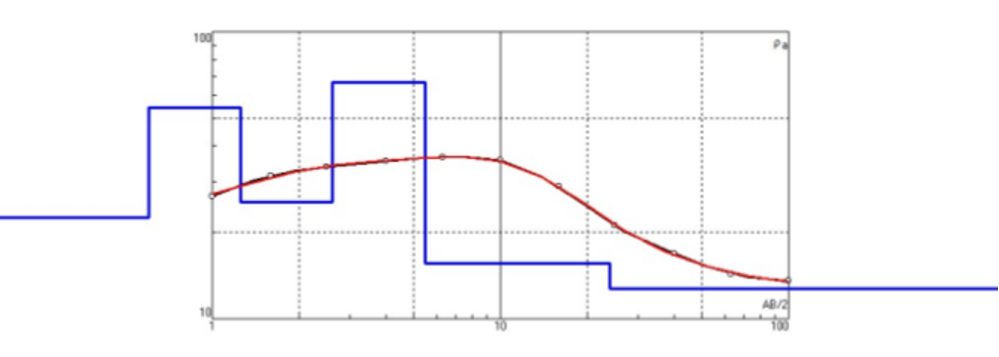
\includegraphics[width=0.8\textwidth]{fig/Schlumberger_5Schichten.pdf}
\caption{Inversionsmodel mit fünf Schichten}
\label{abb:Schlum2}
\end{figure}
%%%%%%%%%%%%%%%%%%%%%%%%%%%%%%%%%%%%
%%%%%%%%%%%%%%%%%%%%%%%%%%%%%%%%%%%%
\begin{figure}[h]
\centering
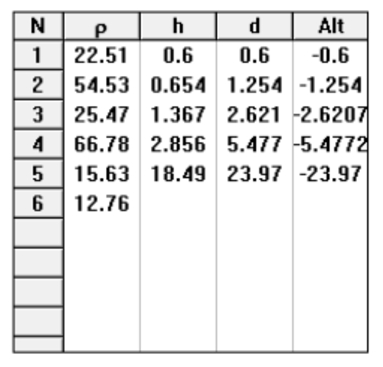
\includegraphics[width=0.3\textwidth]{fig/schlumbergerTabelle2.pdf}
\caption{Datem zum Inversionsmodel mit fünf Schichten. $roh$ bezeichnet den spezifischen Widerstand in $\Omega$m, $h$ die Schichtdicke in m, $d$ die Schichttiefe in m}
\label{abb:SchlumTab2}
\end{figure}
%%%%%%%%%%%%%%%%%%%%%%%%%%%%%%%%%%%%





